\documentclass[border=10pt]{standalone}

\usepackage{tikz}
\usepackage{tikzsymbols}
\usetikzlibrary{calc,patterns,shapes.geometric}

\def\centerarc[#1](#2)(#3:#4:#5){\draw[#1] ($(#2)+({#5*cos(#3)},{#5*sin(#3)})$) arc (#3:#4:#5);}

\begin{document}
	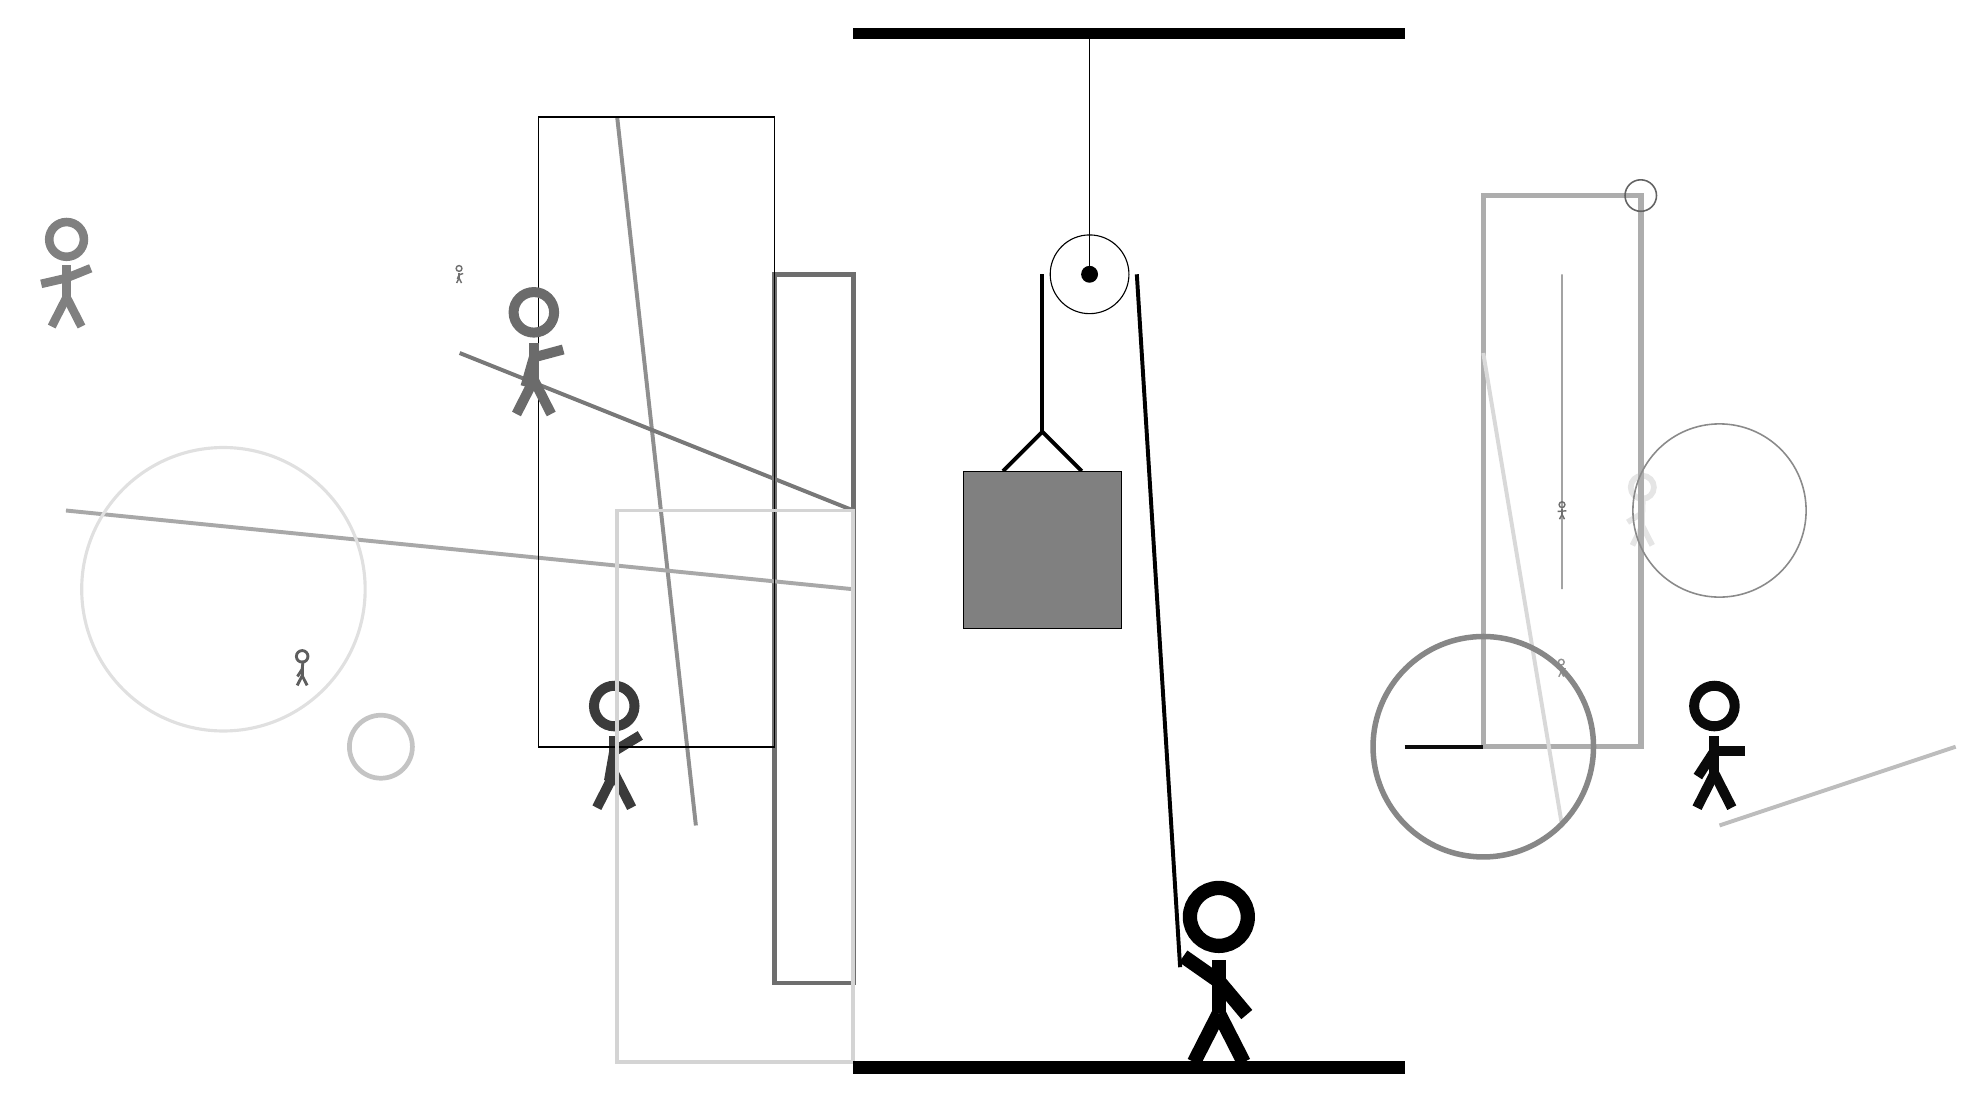
\begin{tikzpicture}
		%%%%% START %%%%%
		
		\draw[fill=black] (-2, 10) rectangle (5, 10.125);
		
		\node[line width=0.7mm, color=black!43] at (7, 2) {\Strichmaxerl[1][79][0]};
		
		\node[line width=0.3mm, color=black!10] at (8, 4) {\Strichmaxerl[4][32][88]};
		\draw[line width=0.5mm, color=black!44](-5, 9) -- (-4, 0);
		\draw[line width=0.6mm, color=black!57] (-2, -2) rectangle (-3, 7);
		\draw[line width=0.5mm, color=black!34](-2, 3) -- (-12, 4);
		\node[line width=0.5mm, color=black!77] at (-5, 1) {\Strichmaxerl[7][80][31]};
		\node[line width=0.4mm, color=black!96] at (9, 1) {\Strichmaxerl[7][57][0]};
		
		\node[line width=0.4mm, color=black!63] at (-9, 2) {\Strichmaxerl[2][57][84]};
		\draw[line width=0.7mm, color=black!32] (6, 1) rectangle (8, 8);
		\draw[line width=0.3mm, color=black!36] (7, 7) rectangle (7, 3);
		\draw[line width=0.5mm, color=black!26](9, 0) -- (12, 1);
		\draw [line width=0.6mm, color=black!23](-8, 1) circle (0.4);
		\node[line width=0.2mm, color=black!57] at (7, 4) {\Strichmaxerl[1][4][4]};
		
		\draw[line width=0.5mm, color=black!53](-2, 4) -- (-7, 6);
		\node[line width=0.7mm, color=black!56] at (-7, 7) {\Strichmaxerl[1][67][19]};
		\draw[line width=0.2mm, color=black!100] (-3, 1) rectangle (-6, 9);
		\node[line width=0.4mm, color=black!50] at (-12, 7) {\Strichmaxerl[6][13][22]};
		\node[line width=0.2mm, color=black!58] at (-6, 6) {\Strichmaxerl[7][74][15]};
		\draw[line width=0.5mm, color=black!15](6, 6) -- (7, 0);
		\draw[line width=0.5mm, color=black!17] (-2, 4) rectangle (-5, -3);
		\draw [line width=0.2mm, color=black!61](8, 8) circle (0.2);
		
		\draw [line width=0.2mm, color=black!46](9, 4) circle (1.1);
		
		\draw[line width=0.5mm, color=black!83](-2, 1) -- (-2, 1);
		\draw [line width=0.4mm, color=black!12](-10, 3) circle (1.8);
		\draw[line width=0.5mm, color=black!95](5, 1) -- (6, 1);
		
		\draw [line width=0.7mm, color=black!47](6, 1) circle (1.4);
		
		\draw (1, 7) circle (0.5);
		\draw[fill=black] (1, 7) circle (0.1);
		\draw (1, 10) -- (1, 7);
		
		\draw[line width=0.5mm] (-0.1, 4.5) -- (0.4, 5.0) -- (0.9, 4.5);
		\draw[fill=black!50] (-0.6, 4.5) rectangle (1.4, 2.5);
		
		\draw[line width=0.5mm] (0.4, 7) -- (0.4, 5.0);
		\centerarc[line width=0.5mm](1, 7)(0:180:0.6);
		\draw[line width=0.5mm](1.6, 7) -- (2.15, -1.8);
		
		\node at (2.6, -1.9) {\Strichmaxerl[10][-35][-50]};
		
		\draw[fill=black] (-2, -3) rectangle (5, -3.15);
		
		%%%%% END %%%%%
	\end{tikzpicture}
\end{document}